% \setcounter{chapter}{-1}
\chapter* {续章}



在日常生活中,当提及人工智能,许多人脑海中可能会浮现出像图\ref{想象中的人工智能}中那样画面:有一个可爱的机器人在房间里热情地跟你打招呼,仿佛是一位贴心的管家;到了饭点,它在厨房中熟练地搅拌锅中的食材,烹饪美味佳肴;当人们享用完美食后,它又将碗碟收拾好,到水池边清洗;亦或是用灵巧的手在帮忙整理床铺,让房间整洁如新。这些场景似乎勾勒出了人们想象中人工智能的模样,充满了科幻感与趣味性。

然而,实际上,人工智能的形态和应用远比这些想象更加丰富多样且贴近人们的生活。它可能隐藏在日常使用的手机语音助手背后,默默地为安排日程、解答疑问;也可能存在于电商平台的推荐系统中,根据用户 的浏览和购买习惯,精准地推送用户可能感兴趣的商品;还可能融入到交通信号灯的控制系统里,优化城市交通流量,减少拥堵人工智能已经在不知不觉中渗透到生活的各个角落,并持续改变着人们的生活方式。

2022年,ChatGPT的出现引发了全球范围的关注,成为人工智能领域的一个标志性事件,其影响力远远超出了技术圈,渗透到了教育、商业、媒体等多个行业。它以强大的自然语言处理能力和生成能力,彻底改变了人们对传统AI助手的认知,重新定义了人机交互的方式,甚至对某些职业的工作模式产生了深远影响。

2025年,DeepSeek的出现又再次掀起人工智能的热潮,引发了一场生产力变革。开源的DeepSeek不仅在技术上实现了跨越式突破,还在应用场景、商业化模式和社会影响上展现了更强大的潜力。各大互联网公司、云厂商、芯片厂商、政务部门等纷纷宣布接入或适配DeepSeek,一款国民级的人工智能应用就此诞生。从身边的种种改变不难看出,人工智能正以不可阻挡之势,全面渗透着人们的生活,助力各行各业的发展。




\begin{figure}[htb]
	\centering
	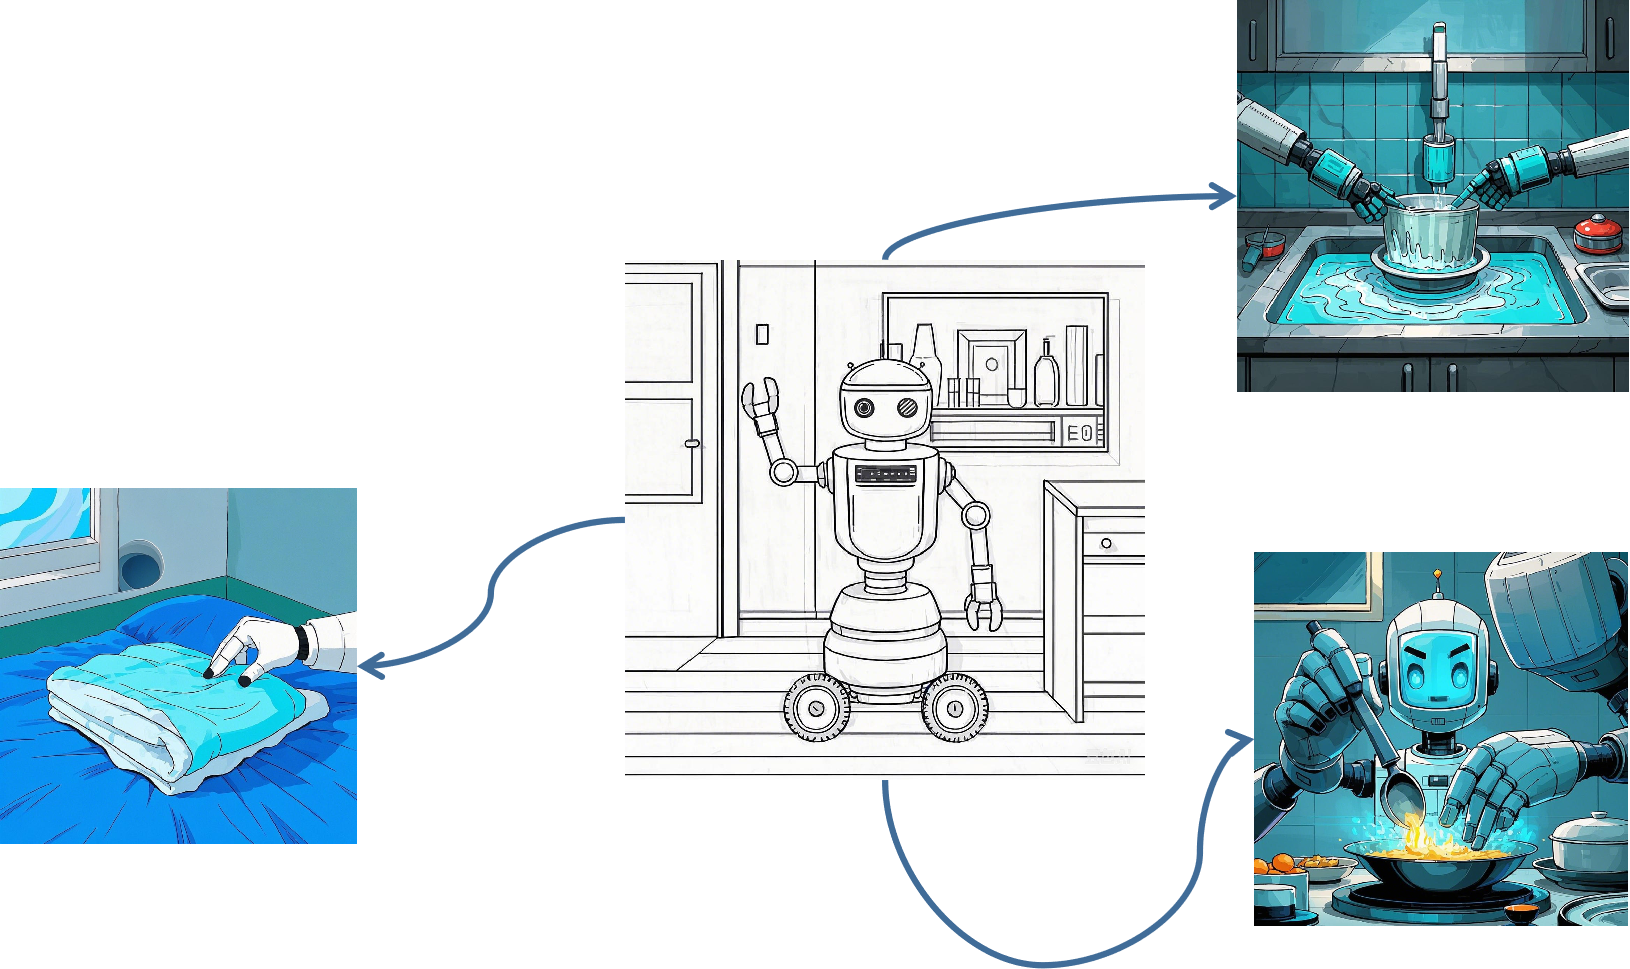
\includegraphics[width=\linewidth]{image/0/想象中的人工智能.png}
	\caption{想象中的人工智能 (图片由 AI 生成)}
        \label{想象中的人工智能}
\end{figure}

\subsubsection*{\textbf{生活中的人工智能}}

要在人们的日常生活中探寻人工智能的踪迹,也许可以从清晨的闹钟说起。第一台个人机械闹钟发明于1787年,它可以在每天凌晨的四点钟准时响起。而闹钟演化至今已有出现了各种功能和形态。人们现在用得更多的闹钟其实是内置在手机里的APP,这些已经十分成熟的闹钟APP,除了更加便捷外,也更加智能了。现在有一些闹钟APP可以通过记录用户平时的睡眠习惯和起床困难程度,给用户量身定做闹铃音乐、给出起床时间的建议。这些都依赖于人工智能的算法,更先进的算法,能给客户更加科学、定制化的闹铃体验。

2024年10月,任天堂发布了一款形态可爱的交互式闹钟Alarmo。它的一切设计都是为了让起床变得更加有趣,所以除了闹钟最基本的操作按钮外,闹钟里面还内置了的运动传感器,可以识别到监测并识别人的动作、手势。它的闹铃服务分为多个阶段,如果传感器识别到用户在前一阶段的闹铃结束后仍然躺在床上,它会切换播放更让人紧张、激烈的闹铃音乐,灯光效果也会逐次变化,直到识别到用户离开床才会停止,甚至还会放一段庆祝的音乐。而姿态的识别离不开人工智能。机器能读懂用户的姿态才能进行下一步的决策。这台闹钟甚至可以在用户起床又犯懒回到床上时,进行二次叫醒。除了基本的叫醒功能,Alarmo还可以通过分析睡眠模式,推算出最佳的起床时间。它考虑了用户习惯、日历事件,甚至天气预报,这样可以让用户醒来时神清气爽,迎接新的一天。这种高度个性化定制都得益于人工智能算法,这些算法会随着时间推移不断学习并做出调整。

\begin{figure}[htb]    
	\centering
	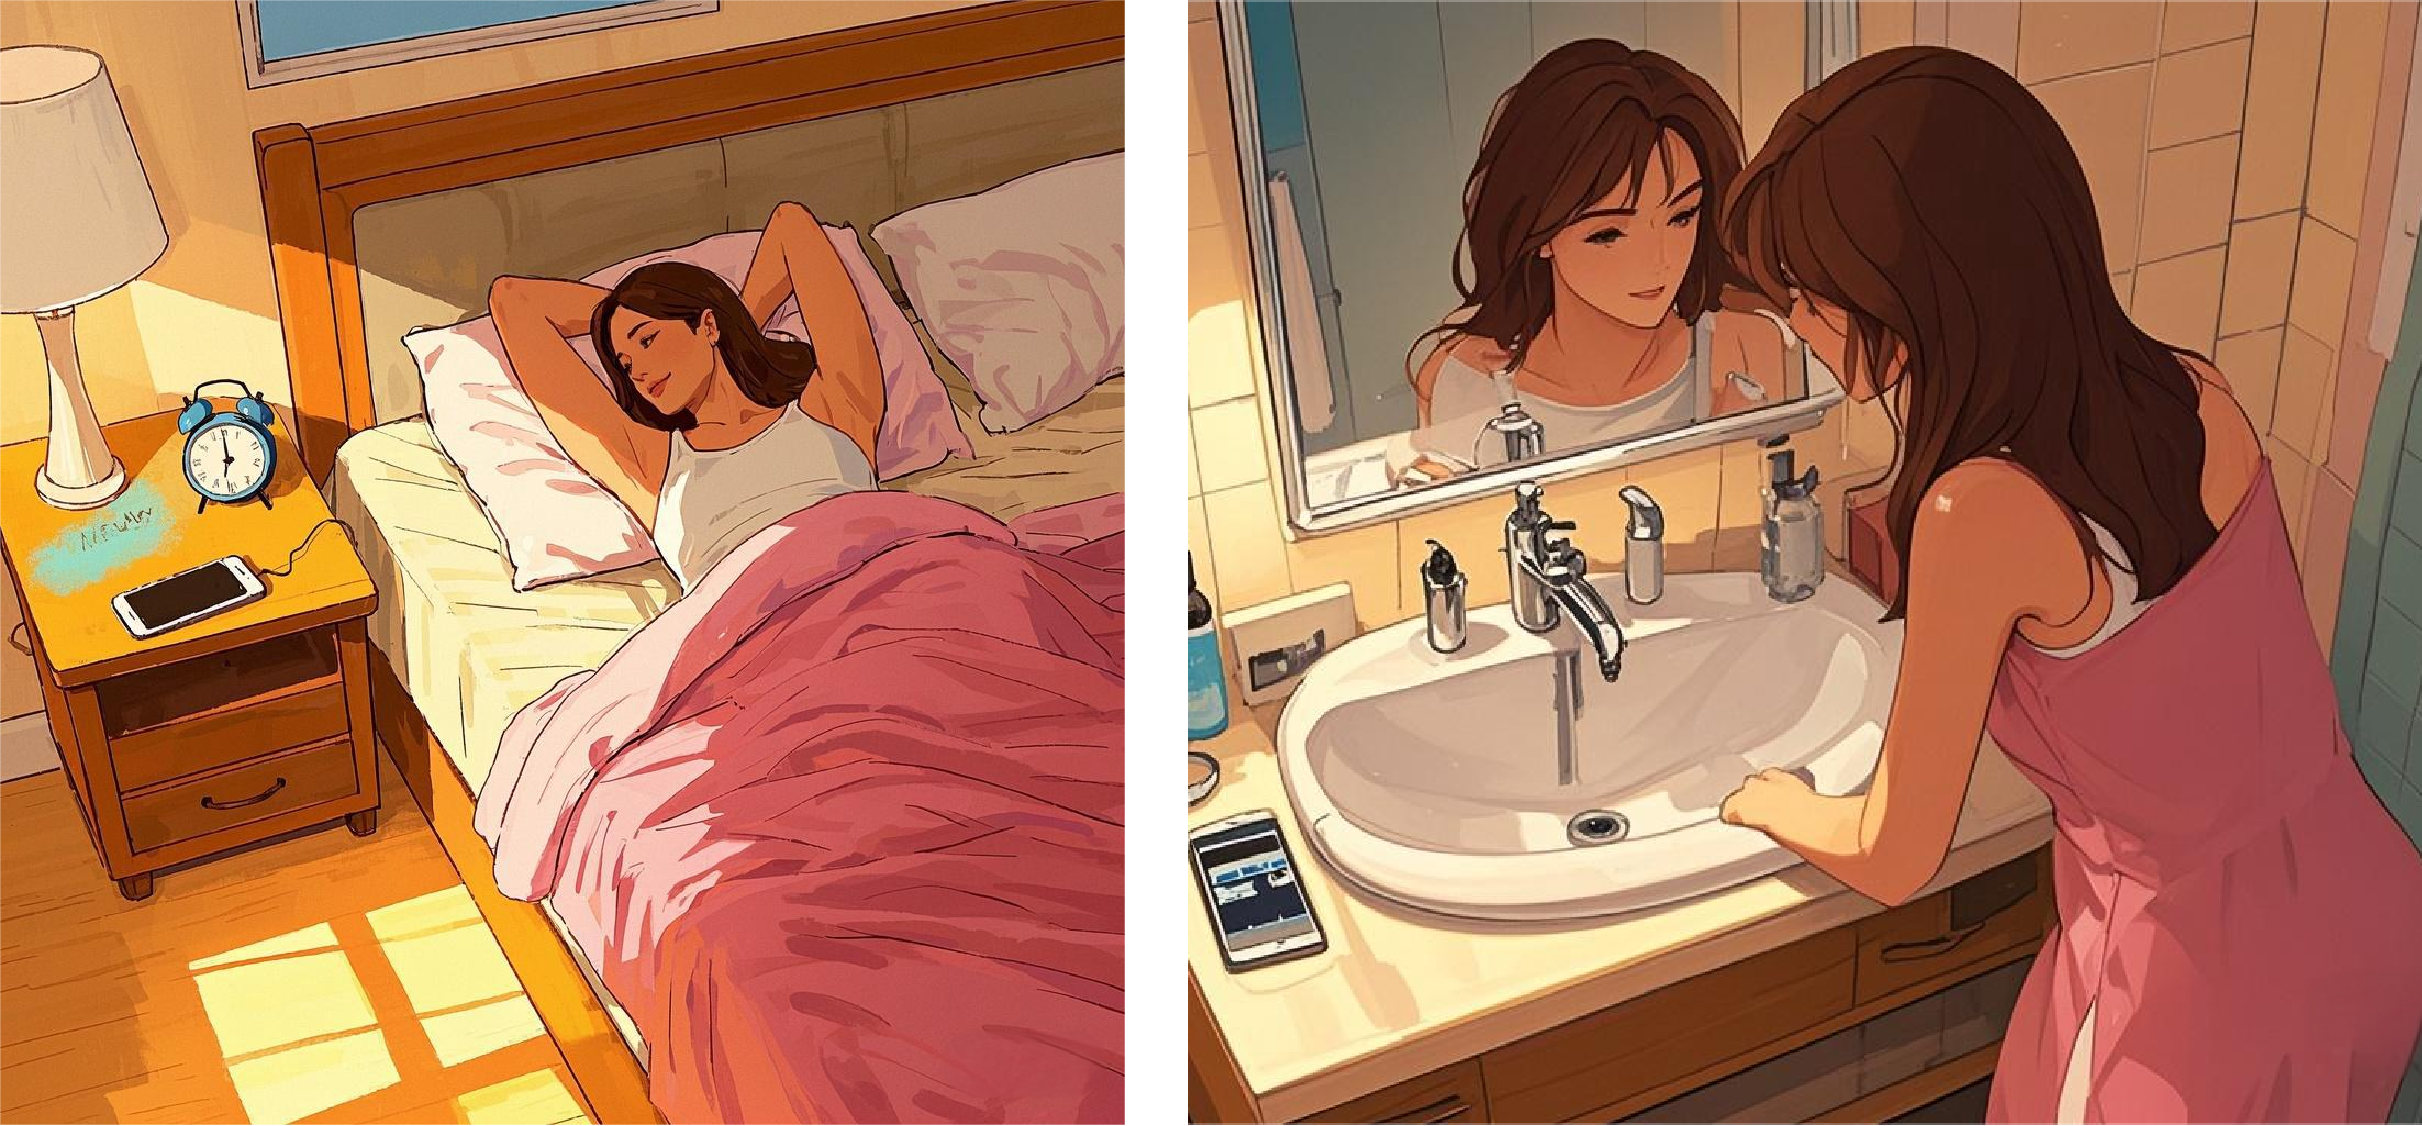
\includegraphics[width=\linewidth]{image/0/清晨.png}
	\caption{清晨的闹铃和音乐播放都有人工智能陪伴 (图片由 AI 生成)}
\end{figure}

起床后的无聊洗漱时间也许会希望伴随着音乐的播放来缓解疲乏。现在的音乐APP除了基本的随机播放、循环播放外,还有一种特殊的播放模式——“心动模式”,它好像总能播放到用户当下想要听的歌。这个功能的实现其实也依赖于人工智能的算法。每个人在互联网上的行动都构成了一幅用户画像,基本用户信息构成了APP对用户最初的认知。而在用户使用的过程中,APP会通过用户的轨迹不断地学习用户的行为,比如用户最近常听的歌曲、曲风的喜好、歌手的喜好、语种的选择等等,再利用大数据推荐相似的歌曲。有的算法还会将天气、时间和地域等因素考虑进去,让歌曲的播放选择更加智能。比如在清晨洗漱时播放的歌曲可能是更偏向明朗轻快风格的歌曲,让人们昏沉的大脑跟随节奏清醒过来。而在夜晚可能更加偏向于播放舒缓轻柔的音乐,让人们能够跟随音乐缓缓进入梦乡。有的音乐APP还有运动模式,可以为用户找到适合不同运动频率的音乐,适配快跑和适配瑜伽的当然是不同种类型的音乐,通过音乐来辅助运动,让一些单人运动不再无聊。

除了能猜到用户的想听什么,音乐APP还能为用户找到音乐的名字。这个功能一般就是听歌识曲,更近一步的还有哼歌识曲。前者是直接听机器外放的音乐来进行识别,比较适合人们在外面偶然听到了某首好听的歌曲,想知道名字,于是立马拿出手机进行听歌识曲,而后者则是人哼唱旋律让APP进行识别,这会更难,所以准确率通常没有听歌识曲高。这里都用了人工智能中的音频识别技术。这个技术让机器能够“听懂”音乐,通过音频的识别与分析,找到与其相近的歌曲,并将结果反馈给用户。



洗漱完毕后,就该踏上上班或上学的道路,无论是开车还是走路,人们总是会用地图导航APP来为自己找到适合的路线。导航APP会根据起点和终点为用户推荐不同的路线。当然,仅仅根据起点和终点是不够的,人们更加希望APP能给出更符合当前路况的实时推荐。所以地图导航APP其实还会结合时间、车流量等实时的路况来进行方案的调整。当然,用户的习惯也是很重要的一个因素,所以选择熟悉的路段也是APP推荐路线的一种偏向。这些元素都是人工智能的路线推荐算法输入,而输出的则是APP对于路线的分析与选择。

当人们讨论哪款地图导航APP更加“智能”的时候,其实更多的是在讨论它推荐的路线是不是更加贴近现实情况,更能让用户在更加快捷、舒服的状态下抵达目的地。地图导航APP发展至今,已经可以做到为用户推荐精细到车道这个程度的方案了,让用户尽早地远离拥堵路段、车道,所以导航语音常伴着一句“您已行驶在最佳路线上。


除了路线外,地图导航APP还会显示实时的交通信号灯的信息,在用户等待红灯时,为其展示“读秒”倒计时。这个功能听起来只需要接入交管系统,让其为APP提供数据就行了,但在现实中要实现会难得多。首先,各个省的交管系统是不互通的,要将这些不同系统的信息整合起来是个大工程。其次,只通过笼统的规则信息推算是不够的,要能做到“读秒”如此精细的程度,需要让交通信号灯联网,才能上传实时的数据,让APP的信息和实际的信号灯同步。但是要让如此庞大数量的信号灯都联网又是巨大的工程量,无论是后建的信号灯要设计联网功能,还是改造原来的老旧信号灯,全部变成智能信号灯,都不是一件容易的事情。

所以在交通信号灯全面达成“智能化”前,地图导航APP是如何实现信号灯的“读秒”呢?答案是人工智能的预测算法。交通信号灯本身具有预设的运行机制,通常遵循固定周期或根据车流量进行调整。导航APP通过采集匿名用户的行车数据(如车辆启停状态、位置移动轨迹),结合历史信号周期规律和实时交通流变化,运用人工智能算法推算出倒计时预测值,从而不断缩小倒计时预测值与真实值之间的偏差。当然,这毕竟是根据用户行为和道路状况进行推算的预测算法,总会有和实际偏差的时候,所以APP上显示的秒数和实际看到的秒数不完全一致也是常常会发生的事情。

到达目的地后,上班族要做的第一件事情是打卡。现在常用的打卡方式是指纹打卡和刷脸打卡。这里以人脸打卡为例。在一个打卡机器前站立,它瞬间就能识别到用户脸的位置并框选出来,并显示识别到的用户的信息。这里面使用到的人工智能技术其实分为两个,一个是人脸检测,一个是身份识别。前者是在摄像头捕获到的画面中检测到是否有人脸,并得到它的位置信息。而后者则是在前者的基础上,识别人脸区域内的这个人具体是这个公司中的哪一位工作人员。根据安全等级的不同可能会用不同摄像头与算法,比如安全等级较低的打卡可能是2D的彩色图像作为输入源进行识别。而进入一些机密区域则需要深度相机拍摄的深度图像作为输入源,并使用更好的算法来得保证更高的识别率。智能手机的人脸解锁其实也是用了同样的技术,所以在人们睁开眼看到看手机的第一眼就已经在享受人工智能技术带来的便利了。


\begin{figure}[htb]
	\centering
	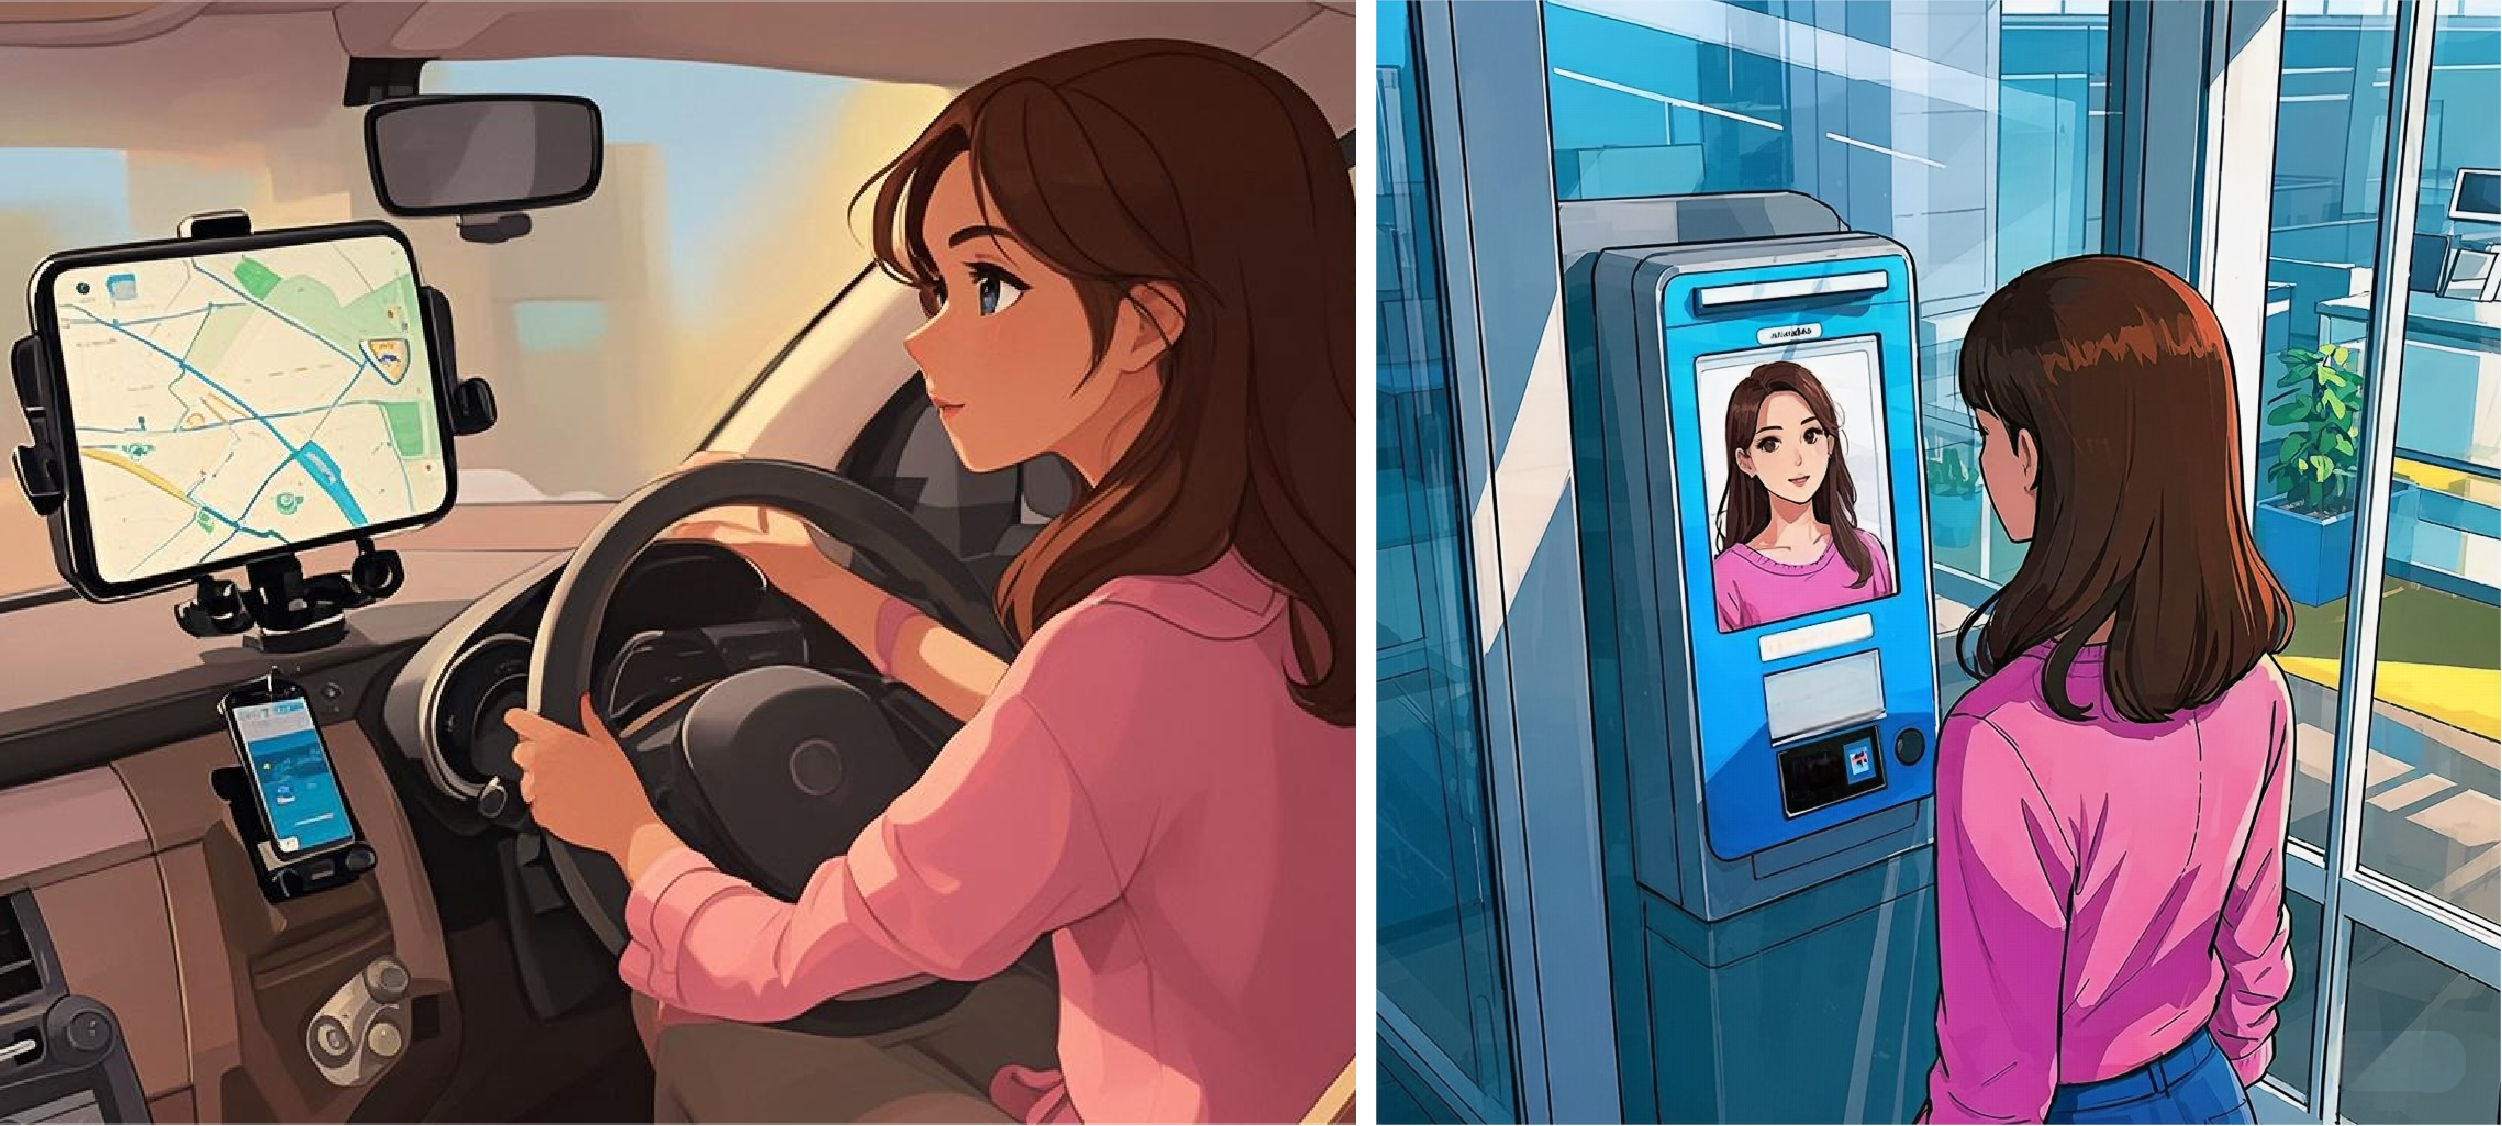
\includegraphics[width=\linewidth]{image/0/上班.png}
	\caption{智能导航与人脸识别打卡 (图片由 AI 生成)}
\end{figure}


工作学习时,总会遇到让人苦恼的难题,人们总是在寻找让学习工作更智能化的方式。而现如今,人工智能助手带来了巨大的工作方式变革。早期的智能语音助手内置在手机中,为生活安排提供帮助,它们能做到事情很有限,例如打电话、定闹铃、打开APP等,但是简单的功能其实也用到了人工智能的技术,比如语音识别,手机需要在听到音频时,用算法识别出来这是一条指令,才能做后续的事情。后来大模型智能时代来临,智能助手的定义变得更加宽泛,人们对它的使用频率也显著增加。

一个标志性的产品是前文所提到的DeepSeek,用户可以在对话框中与它聊天来寻求问题的答案。和以往普通的对话助手不同,它并不是只依赖于“关键词”的触发。而且更像是“理解”了人们说的话之后才给出相应的答案。让机器能“看懂”用户的文字,这就用到了人工智能中的自然语言处理技术。而机器要生成答案给用户则还结合了的生成式人工智能技术。这些技术会在本书的后续章节中逐一为大家讲解。人工智能助手可以处理非常多事情,例如生成一份个性化定制的菜谱,或是帮助用户生成实现某种功能的代码,还可以生成报告等文章。总之,遇到难题尝试问一问人工智能助手,也许能提供灵感或解决问题。

近些年,智能助手飞速发展,已经可以做到处理多种数据源的输入并输出多种类型的回答,这就是多模态。除了文字的解答,现在的智能助手还能与用户进行自然地通话,甚至能通过语气判断用户的情绪给出不一样的对话结果。利用人工智能中的音频生成技术,可以生成不同性别、口音、语气,停顿自然的语音回答,让人们感觉更像在和一个“真人”交谈。这样智能又自然的交互方式衍生了出了许多种用法,例如让人工智能助手充当英语老师,陪用户练习口语,实时地纠正错误的语法和读音。还有扮演面试官,锻炼用户的面试技巧,也能让用户在模拟中学习到更多面试技巧,在实际面试中发挥得更好。

\begin{figure}[htb]
	\centering
	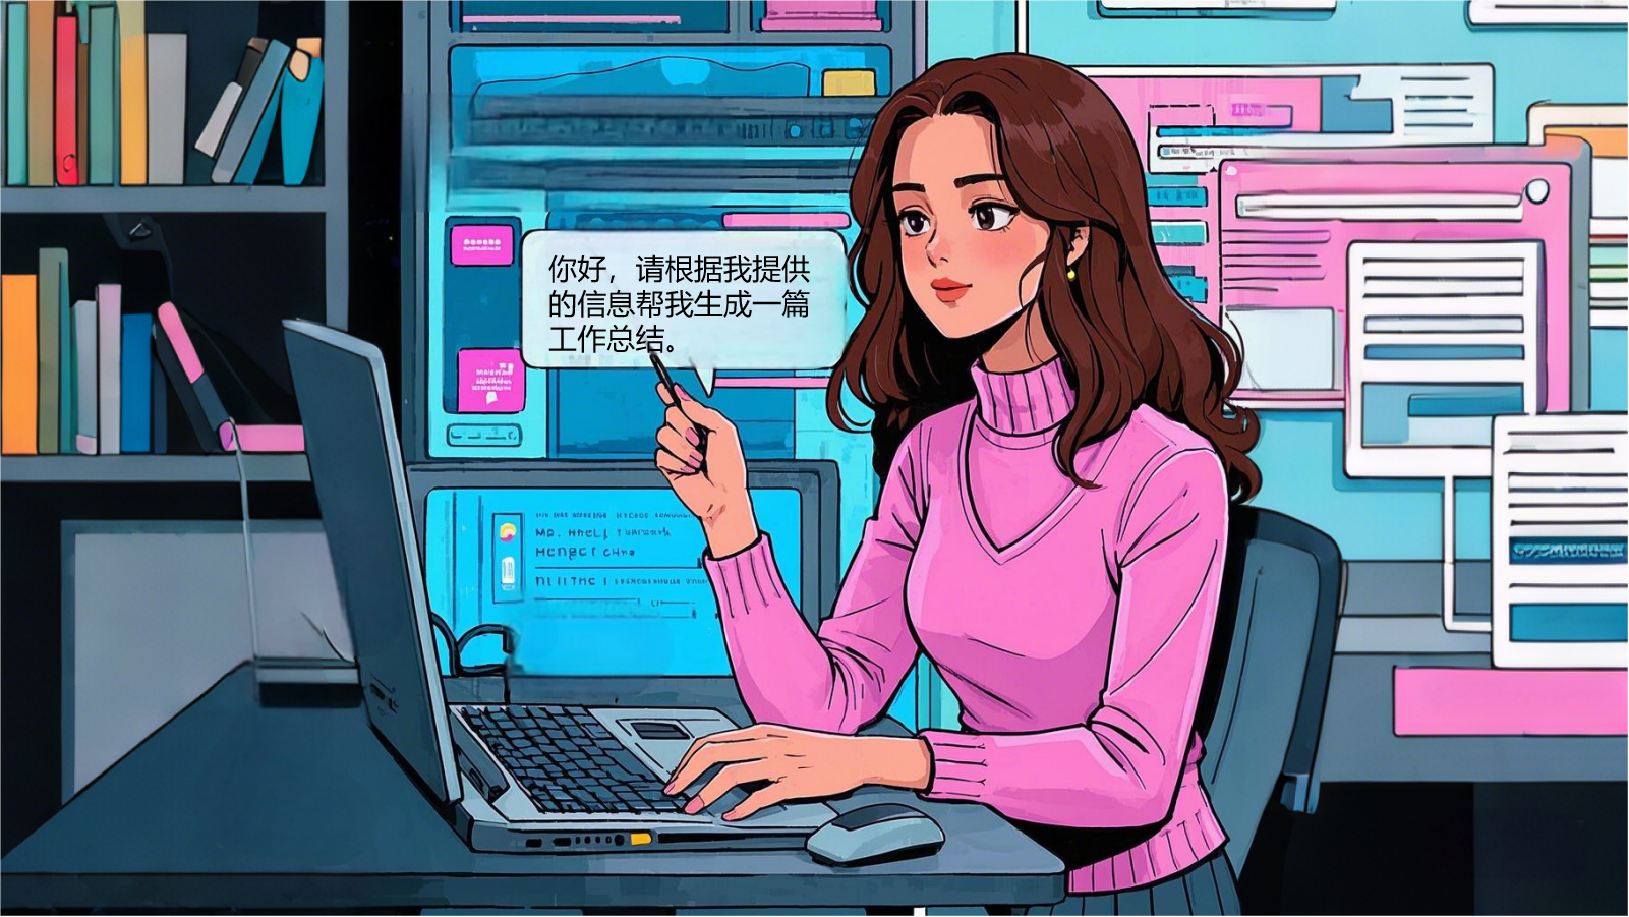
\includegraphics[width=\linewidth]{image/0/智能助手.png}
	\caption{让智能助手生成工作总结 (图片由 AI 生成)}
\end{figure}

除了工作和学习,娱乐领域也处处是人工智能的身影。为了吸引用户持续地使用APP,各类社交娱乐APP总是会将用户感兴趣的内容推送到首页。这和前面的音乐APP是类似的原理。APP在利用人工智能算法不断地学习用户的喜好,根据搜索历史、停留时间、评论点赞收藏等互动信息等,将用户的画像进一步刻画,推送用户更喜欢的东西。所以人们会发现一当频繁点击或者最近搜索过某些内容后,首页刷新出来的大多是和这些关键词相关的内容。而用户在一段时间不去点击互动相关信息,或者主动是按下“不感兴趣”的按钮后,这些内容出现频率又降低了。所以人们总会感觉刷视频停不下来,因为人工智能和大数据在不断地推送吸引力高的内容,让人们留在APP里消耗时间。

购物APP中的“猜你想买”也是用了类似的技术,APP根据用户最近搜索浏览的物品、买过的物品、收藏过的物品、购物车中的物品等等信息来预测用户可能想买的东西,展示给用户,以此来刺激消费。所以每个人的购物APP首页都是不一样的,甚至搜索结果页面也是不一样的。同样的关键词搜索出来的内容,会根据用户的消费水平和喜好有所调整,所以不同人搜索同样的东西,展示出来的商品差别很大也不足为奇了。

还有购物APP中利用人工智能的虚拟试衣技术,让消费者无需亲自试穿,就能在屏幕上直观看到不同款式、颜色的服装穿在自己身上的效果。通过对用户身材数据的精准采集和 3D 建模技术,再结合人工智能算法,系统能够模拟出服装的真实穿着形态和动态效果,极大地提升了购物的便捷性与趣味性,同时也减少了因尺码、款式不合适而导致的退换货情况。

\begin{figure}[htb]
	\centering
	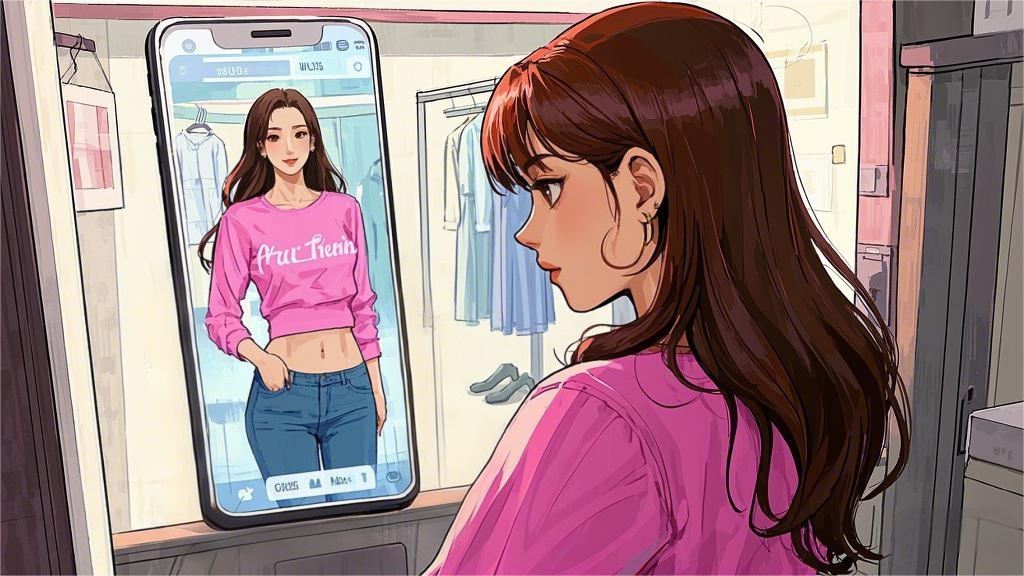
\includegraphics[width=\linewidth]{image/0/虚拟试衣.png}
	\caption{虚拟试衣功能让人们能直观地看到衣服穿在自己身上的样子 (图片由 AI 生成)}
\end{figure}

还有一些娱乐相关的“黑科技”,其实也是因为加入了人工智能的助力才会如此便捷和神奇。比如一些P图软件可以一键去除水印、区域重绘、抠图、物体消除、人物特效等等,这些功能都用了计算机视觉相关的技术。处理出来的图片比以前更自然更真实,也更贴近用户的需求,让一些曾经需要专业图像处理技术或是绘画技术才能满足的需求,现在能够“傻瓜式”地一键完成。

再例如一些可以发弹幕的视频软件。当一个视频弹幕太多了,可能会遮挡住视频的主体内容,带来不好的体验。现在有了弹幕环绕模式,弹幕会飘在视频主体人物周围,在关键区域就隐藏了起来,就像把人物扣了出来,提高了一个图层。这样既不影响视频内容的观看,又不会错过有趣的弹幕讨论。

\begin{figure}[htb]
	\centering
	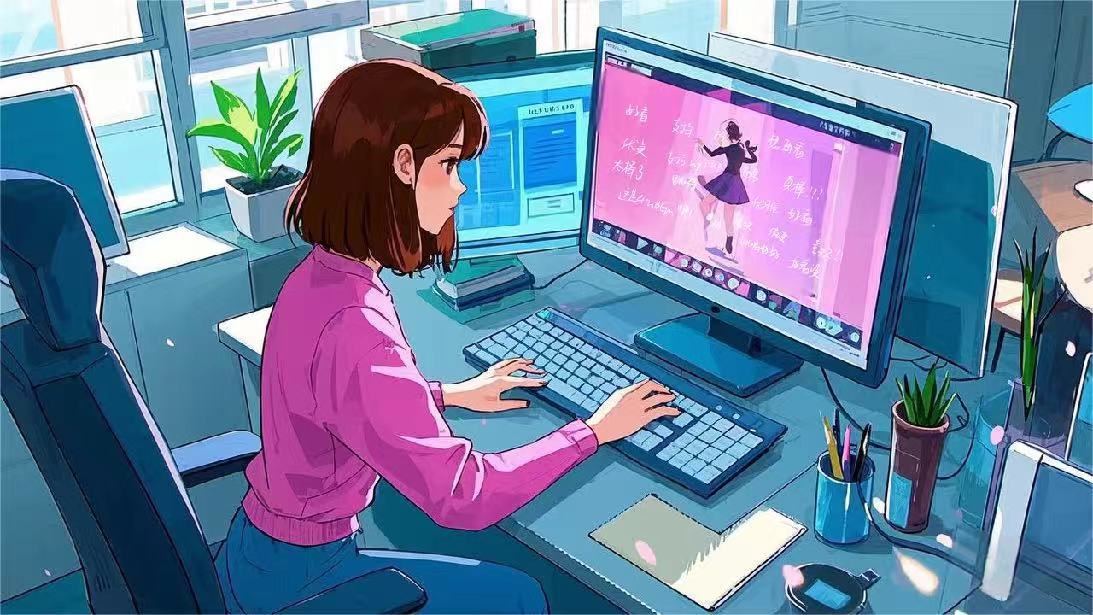
\includegraphics[width=\linewidth]{image/0/弹幕.jpg}
	\caption{视频弹幕环绕模式,不遮挡人物 (图片由 AI 生成)}
\end{figure}


人工智能技术已经渗透进了人们衣食住行的每个角落。从清晨被智能闹钟唤醒,到伴着契合心情的音乐洗漱,再到依靠精准导航奔赴目的地,工作学习时借助智能助手排忧解难,休闲娱乐时沉浸于个性化推送带来的愉悦体验,人工智能正以润物细无声的方式,全方位地重塑着人们的生活。它不仅改变了人们的生活方式,更拓宽了人们对未来生活的想象空间。它让人们的生活变得更加高效、便捷、舒适和丰富多彩。
% https://36kr.com/p/2159359924936451

% 换一双发现人工智能的眼睛,跟着小欣度过她和人工智能息息相关的一天。小欣是一个上班族,清晨她在智能闹钟的轻柔音乐中醒来,这闹钟可不是普通的计时器,它通过学习小欣过往的睡眠数据,在最合适的浅睡阶段将她唤醒,让她能精神饱满地开启新的一天。小欣开始洗漱,为了打发漫长的收拾时间,她打开了音乐播放器,按下了播放按钮,音乐播放器利用推荐算法,结合现在的时间和她以往的听音乐习惯为她播放了一首略带动感的音乐,让她懒散的身体逐渐跃动了起来。梳妆完毕,小欣从家里出发,她打开地图软件,根据时间短自动推断出她现在要去公司,于是将公司作为目的地放在了她路线的第一条。她坐上驾驶座,发动车子,跟随导航开上了上班的道路。

% 智能导航检测到小欣正在行驶在熟悉路段,于是自动减少了提醒的频率,她感觉清净了许多。但不巧的是,这条熟悉的路上恰好出了车祸,道路变得异常堵塞。导航软件立刻使用智能算法,为她推荐了其他时间更短的路径,由于另一条路是小欣从未走过的,导航软件增加了提醒的频率,并时刻为小欣提供最佳车道的信息。有了智能导航的帮助,小欣按时到达了公司。公司员工需要统一用某款软件进行签到,这个软件利用手机的GPS定位,保证员工在公司200米以内才能开启签到,并且使用人脸识别技术进行双重签到保障。

% 小欣来到工位上,打开了她的电脑。还未到上班时间的她准备看一下新闻,网页已经非常智能地为她整理了一些重要的新闻以及她可能感兴趣的新闻消息供她查阅,根据她点击的选择和阅读的时长信息,新网网页又再一次地更新了属于她的用户画像与推荐标签,让下一次的整理更符合她的心意。


% 小欣到了家门口,她将大拇指放在家门口的指纹锁上,指纹锁通过图像识别技术,匹配到这是主人的指纹,将门锁打开。小欣家的指纹解锁还可以


\subsubsection*{\textbf{本教材内容概述}}
本书作为一本通识类课程教材,适用于所有专业的本科生、研究生,以及对人工智能感兴趣,希望入门的读者。本教材旨在引导读者了解人工智能的基础概念、技术原理及其广泛的应用场景。为读者提供一个关于人工智能的全面视角,从基础理论到技术实践,再到伦理考量,涵盖了人工智能的全貌。

本书首先从计算的渊源讲起,探索智能行为的起源,进而介绍人工智能的分类和发展历程,并讨论人工智在现代社会中的应用。教材深入探讨了机器学习、深度学习等人工智能基础概念,以及计算机视觉和自然语言处理等核心技术,为读者提供了坚实的技术基础。通过广泛且贴近生活的例子,让读者能够对身边的人工智能有更加深刻的认识,感受人工智能在身边带来的便捷与变革。通过实践案例,如图像分类项目,读者将亲自参与到数据集的处理、模型的选择、训练、评估等环节中,以加深对AI技术应用的理解。
本书不仅关注技术本身,还关注技术对社会的影响。通过讨论创新发展与社会影响、算法歧视、隐私忧虑、责任与安全以及机器人权利等问题,旨在引导读者多方位地思考人工智能带来的伦理挑战,培养社会责任感和伦理意识。培养国家认同感和社会责任感。